
\subsection{Napkin Math and Synthetic Margins}

The bar was dim, upscale but unpretentious. It was the kind of place where the lighting was low enough to suggest intimacy, 
but not so low that you couldn’t read a term sheet. A jazz trio murmured in the corner, and the leather booths smelled 
faintly of cedar and citrus polish.

Hart pulled a cocktail napkin toward him and clicked a pen from his jacket. He didn’t bother asking for a fresh sheet of paper.

``Let’s run the numbers,'' he said, scribbling a row of assumptions down the margin. ``Not investor math. 
Fermi math.''

Morales grinned and leaned in. ``Back-of-the-envelope?''

``Always,'' Hart said. ``It’s not about precision. It’s about order of magnitude sanity.''

He drew three columns: headcount, compliance burden, deployment velocity.

``Say a fund with \$300 million AUM wants to scale into synthetic credit. Normally they’d need --- what? --- five 
headcount just to maintain reporting compliance?''

\medskip

\begin{TechnicalSidebar}{What is Synthetic Credit?}

    \textbf{Synthetic credit} refers to exposure to credit risk through financial derivatives—rather 
    than through direct ownership of bonds or loans (Choudhry, 2004; Tuckman \& Serrat, 2011).
  
    \medskip
    
    Unlike traditional credit instruments (e.g., corporate bonds), synthetic credit positions are 
    created using tools such as:
  
    \medskip
  
    \begin{itemize}
      \item \textbf{Credit Default Swaps (CDS):}  
      A CDS functions like credit insurance. The buyer pays a regular premium to the seller, and in 
      return, gets compensated if a third-party borrower (like a company or government) defaults 
      (Hull, 2012).  
  
      \medskip
    
      \textit{Example:} It's like paying monthly insurance on a neighbor’s mortgage. However, you don’t 
      own the house, but you’ll get a payout if they default on the loan.
  
      \medskip
  
      \item \textbf{Total Return Swaps (TRS):}  
      In a TRS, one party agrees to hand over the total return (interest + price appreciation) from a 
      credit asset in exchange for a fixed or floating payment (Bomfim, 2005).
  
      \medskip
  
      \textit{Example:} Imagine you own a risky bond, but instead of collecting its unpredictable income, 
      you trade it for steady monthly rent and give someone else the upside (and risk) in exchange for 
      certainty.
  
      \medskip
  
      \item \textbf{Structured Notes or Options:}  
      These are custom-built financial products based on baskets of credit indices or portfolios, often 
      with embedded features like leverage or downside protection (Jobst, 2007).
  
      \medskip
  
      \textit{Example:} Think of it like a chef's tasting menu. You're not just betting on one credit, 
      but on a handpicked combo of bonds or indices, with special ingredients like caps, floors, or 
      trigger conditions that shape how (and if) you get paid.
    \end{itemize}
  
    \medskip
    
    These instruments allow funds to scale exposure rapidly without purchasing underlying assets. 
    They're cheaper, faster, and more capital-efficient—but also more opaque (Partnoy \& Skeel, 2007).
  
  \medskip

  \begin{figure}[H]
    \centering
    \resizebox{0.92\textwidth}{!}{%
      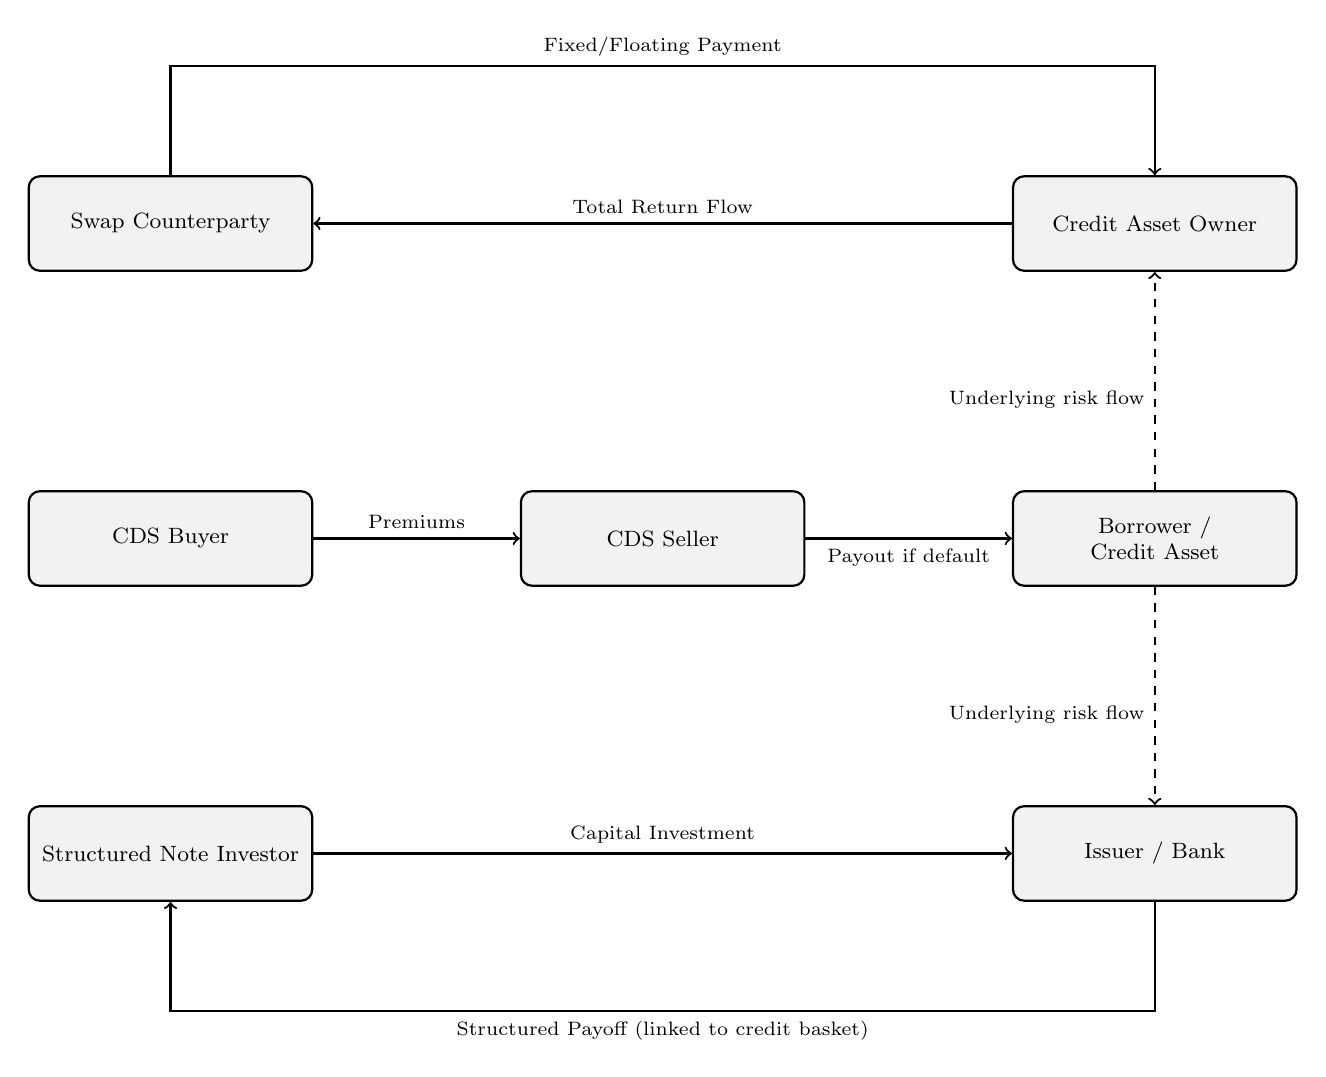
\begin{tikzpicture}[
        font=\footnotesize,
        box/.style={draw, thick, rounded corners, minimum width=3.6cm, minimum height=1.2cm, align=center, fill=gray!10},
        arrow/.style={->, thick},
        note/.style={font=\scriptsize\itshape},
        x=2.5cm, y=2cm
      ]
  
      % Source of risk
      \node[box] (borrower) at (5,0) {Borrower /\\Credit Asset};
  
      % CDS
      \node[box] (cdsbuyer) at (0,0) {CDS Buyer};
      \node[box] (cdsseller) at (2.5,0) {CDS Seller};
  
      \draw[arrow] (cdsbuyer) -- node[above] {\scriptsize Premiums} (cdsseller);
      \draw[arrow] (cdsseller) -- node[below] {\scriptsize Payout if default} (borrower);
  
  
      % TRS
      \node[box] (trsasset) at (5,2) {Credit Asset Owner};
      \node[box] (trsparty) at (0,2) {Swap Counterparty};
  
      \draw[arrow] (trsasset) -- node[above] {\scriptsize Total Return Flow} (trsparty);
      \draw[arrow] (trsparty) 
        -- ++(0, 1) coordinate (drop)
        -- ++(+2.5, 0) coordinate (midpoint)
        -|
        (trsasset);

      \node[above] at (midpoint) {\scriptsize Fixed/Floating Payment} (trsasset);
  
  
      % Structured Notes
      \node[box] (investor) at (0,-2) {Structured Note Investor};
      \node[box] (issuer) at (5,-2) {Issuer / Bank};
  
      \draw[arrow] (investor) -- node[above] {\scriptsize Capital Investment} (issuer);
      \draw[arrow] (issuer) 
        -- ++(0, -1) coordinate (drop)
        -- ++(-2.5, 0) coordinate (midpoint)
        -|
        (investor);
      \node[below] at (midpoint) {\scriptsize Structured Payoff (linked to credit basket)};


  
  
      % Borrower arrow
      \draw[arrow, dashed] (borrower) -- node[below left] {\scriptsize Underlying risk flow} (trsasset);
      \draw[arrow, dashed] (borrower) -- node[below left] {\scriptsize Underlying risk flow} (issuer);

      %\node[note] at (-2,2.6) {CDS shifts default risk};
      %\node[note] at (4,0.8) {TRS swaps performance for certainty};
      %\node[note] at (2.5,-3.3) {Notes repackage risk into custom products};
  
      \end{tikzpicture}%
    }
    \caption{How Credit Derivatives Distribute or Transform Credit Risk}
  \end{figure}

  \medskip
  
  \textbf{Why use it?}  

  \medskip

  Funds deploy synthetic credit to:

  \medskip
  
  \begin{itemize}
    \item Express directional credit views without taking balance sheet risk
    \item Hedge credit portfolios with speed and precision
    \item Amplify leverage in a regulatory-compliant wrapper
  \end{itemize}

  \medskip
  
  \textbf{The tradeoff:}  
  
  \medskip

  While synthetic credit boosts flexibility and velocity, it can distort actual exposure metrics. During stress events, 
  the correlation between synthetic and physical markets can break down—causing ``drift'' between expected protection 
  and realized loss.

  \medskip
  
  This divergence played a central role in multiple financial dislocations, including the 2008 collapse of AIG’s CDS 
  book, and more recently, in smaller liquidity ruptures triggered by undercapitalized synthetic tranches.
  
\end{TechnicalSidebar}

\medskip

``Minimum,'' David said. ``Assuming no turnover.''

``Right,'' Hart said, underlining the number. ``Now suppose your pipeline replaces three of those roles 
and reduces latency by 60\%. What does that buy them?''

``Speed to market. And internal optics.''

Hart nodded. ``And optics translate into allocation. Faster compliance means faster scaling.''

He tapped the napkin, now smudged with numbers and ink streaks.

``That’s your margin,'' he said. ``Not in features. In time arbitrage.''

David stared at the scribbled napkin. The math was loose. But the logic was airtight.

He didn’t need a calculator. He needed a clock.

And Hart had just reset it.

\medskip


\begin{HistoricalSidebar}{Fermi Estimation --- How Atomic Physics Became a Quant Interview Question}

    In July 1945, at the Trinity nuclear test site in New Mexico, Enrico Fermi stood among a group of physicists waiting for 
    history to unfold.  
    As the countdown to the first atomic explosion reached zero, Fermi performed an odd, almost casual act: he dropped small 
    scraps of paper.
  
    \medskip
  
    When the shockwave from the detonation reached him, he observed how far the papers had traveled.  
    From that simple displacement, he estimated the blast yield at approximately 10 kilotons of TNT (Rhodes, 1986).  
  
    \medskip
  
    Official measurements later put it at about 18.6 kilotons — meaning Fermi, with no instruments and only a handful of confetti, 
    was within a factor of 2.
  
    \medskip
  
    This moment became legend: not because of the accuracy, but because of the method.  
    Fermi didn’t measure. He decomposed the problem into approximate parts — what we now call a \textbf{Fermi estimate} 
    (Weinstein \& Adam, 2008).
  
    \medskip
  
    \textbf{Fermi estimation} is a mental technique for approximating a quantity using only logical reasoning and 
    order-of-magnitude assumptions (Mahajan, 2010).  
    It’s the art of going from ``I have no idea'' to ``I have a rough sense'' using structured guesswork.
  
    \medskip
  
    \textbf{The canonical example:}  
    How many piano tuners are there in Chicago?
  
    \medskip
  
    \begin{itemize}
      \item Population of Chicago: \textasciitilde3 million  
      \item Average household size: 2.5 $\Rightarrow$ 1.2 million households  
      \item Households with pianos: \textasciitilde1 in 20 $\Rightarrow$ 60,000 pianos  
      \item Tunings per piano per year: 1  
      \item Total tunings: 60,000/year  
      \item A tuner can do 4 jobs/day, 5 days/week, 50 weeks/year = 1,000 tunings/year  
      \item Needed tuners: 60,000 / 1,000 = \textbf{60 piano tuners}
    \end{itemize}
  
    \medskip
  
    Of course, the real number might be 50 or 80. But that’s not the point.  
    What matters is the \textbf{reasoning} (Poundstone, 2003).
  
    \medskip
  
    That’s why Fermi questions became a staple of quant interviews, startup pitches, and market strategy sessions.  
    They don’t test precision.  
    They test \textbf{decomposition, intuition, and the courage to guess} (Munroe, 2015).
  
    \begin{quote}
    \textit{“All models are wrong,”} the saying goes, \textit{“but some are useful.”}  
    Fermi estimates live in that exact margin.
    \end{quote}
  
    \medskip
  
    Whether estimating nuclear yields or billion-dollar TAMs, Fermi logic reminds us:  
    You don’t need perfect data to make a high-quality decision.  
    You just need the guts to bound the problem — and the clarity to own your assumptions.
  
\end{HistoricalSidebar}
  
  
